\section{Ajuste por cuadrados minimos}

\subsection{Hipotesis}

Para verificar que el algoritmo tiene un tiempo de ejecución de $O(N^2)$, realizamos un ajuste de cuadrados con la siguiente función.

$F(N) = a * N^2 + b$

donde $a$ y $b$, son los parámetros a ajustar.

\subsection{Datos de entrada}

\begin{itemize}
    \item $N$, el tamaño del problema (la cantidad de monedas)
    \item $T(N)$ el tiempo de ejecución para cada cada tamaño N
\end{itemize}

\subsection{Recopilacion de datos}

Para obtener mediciones confiables y reducir el ruido, seguimos los siguientes pasos:

\begin{itemize}
    \item Múltiples tamaños. Probamos con 20 tamaños distintos, espaciados uniformemente entre $n = 100$ y $n = 1.000$ (podemos ver que a diferencia del tp anterior, ahora nuestro rango es mucho menor, esto ya que el algoritmo anterior era lineal y este polinomial).
    \item Múltiples datasets. Para cada tamaño $n$, generamos 10 conjuntos de datos  aleatorios independientes
    \item Promedio de mediciones. El tiempo de ejecución reportado para cada tamaño $n$ es el promedio aritmético de las mediciones obtenidas para ese tamaño.
\end{itemize}   

\subsection{Codigo usado}

\begin{lstlisting}[language=Python]
from util import time_algorithm
from TP2 import elegir

# Siempre seteamos la seed de aleatoridad para que los resultados sean reproducibles
seed(12345)
np.random.seed(12345)

sns.set_theme() 

def get_random_array(size: int):
    return np.random.randint(0, 100.000, size)

def main():
    # La variable x van a ser los valores del eje x de los graficos en todo el notebook
    # Tamanio minimo=100, tamanio maximo=10kk, cantidad de puntos=20
    x = np.linspace(100, 1000, 20).astype(int)

    results = time_algorithm(elegir, x, lambda s: [get_random_array(s)])

    ax: plt.Axes
    fig, ax = plt.subplots()
    ax.plot(x, [results[i] for i in x], label="Medicion")
    ax.set_title('Tiempo de ejecucion de elegir')
    ax.set_xlabel('Tamanio del array')
    ax.set_ylabel('Tiempo de ejecucion (s)')

    # scipy nos pide una funcion que recibe primero x y luego los parametros a ajustar:
    f = lambda x, c1, c2: c1 * (x ** 2) + c2 

    c, pcov = sp.optimize.curve_fit(f, x, [results[n] for n in x])

    print(f"c_1 = {c[0]}, c_2 = {c[1]}")
    r = np.sum((c[0] * (x ** 2) + c[1] - [results[n] for n in x])**2)
    print(f"Error cuadratico total: {r}")
        
    y_medido = np.array([results[n] for n in x])
    y_predicho = c[0] * (x ** 2) + c[1]

    ss_res = np.sum((y_medido - y_predicho)**2)
    ss_tot = np.sum((y_medido - np.mean(y_medido))**2)

    r_cuadrado = 1 - (ss_res / ss_tot)
    print(f"R^2 = {r_cuadrado}")
    
    
    ax.plot(x, [c[0] * (n ** 2) + c[1] for n in x], 'r--', label="Ajuste")
    ax.legend()
    
    plt.show()


if __name__ == '__main__':
    main()
\end{lstlisting}

\subsection{Resultados}

Los resultados del ajuste por cuadrado mínimo son.

\begin{itemize}
    \item $a = 5.174732735449362e-07$
    \item $b = -0.0031624210643063184$
    \item Error cuadrático total $(R) = 0.001397511937062671$
    \item Calidad del ajuste $(R^2) = 0.9972484750254462$
\end{itemize}

\begin{figure}[H]
    \centering
    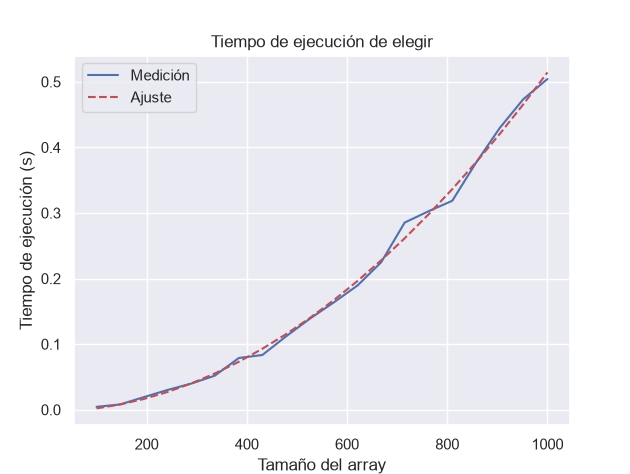
\includegraphics[width=1\textwidth]{img/grafico_analisis.png}
\end{figure}

\subsection{Interpretacion}

Usamos el coeficiente de determinación $R^2$

\begin{itemize}
    \item $R^2 = 1.00$: Ajuste perfecto
    \item $R^2$ mayor $0.98$: Excelente ajuste → Complejidad verificada
    \item $R^2$ mayor $0.95$: Muy buen ajuste → Complejidad muy probable
    \item $R^2$ menor $0.90$: Ajuste pobre → Resultados no concluyentes
\end{itemize}

\subsection{Conclusion}

Con un valor de $R^2 = 0.99$ (mejor que el anterior), concluimos que la complejidad del algoritmo es $O(N^2)$, debido a la alta calidad del ajuste. 